\section{Modelado formal con Redes de Petri}

Para analizar el protocolo 2PC simplificado se modela una única
transacción con un coordinador y un participante. En la Figura
\ref{fig:red-petri-2pc} se muestran los lugares como círculos, los mensajes
pendientes como lugares intermedios y las acciones como transiciones
rectangulares.

\begin{figure}[H]
    \centering
    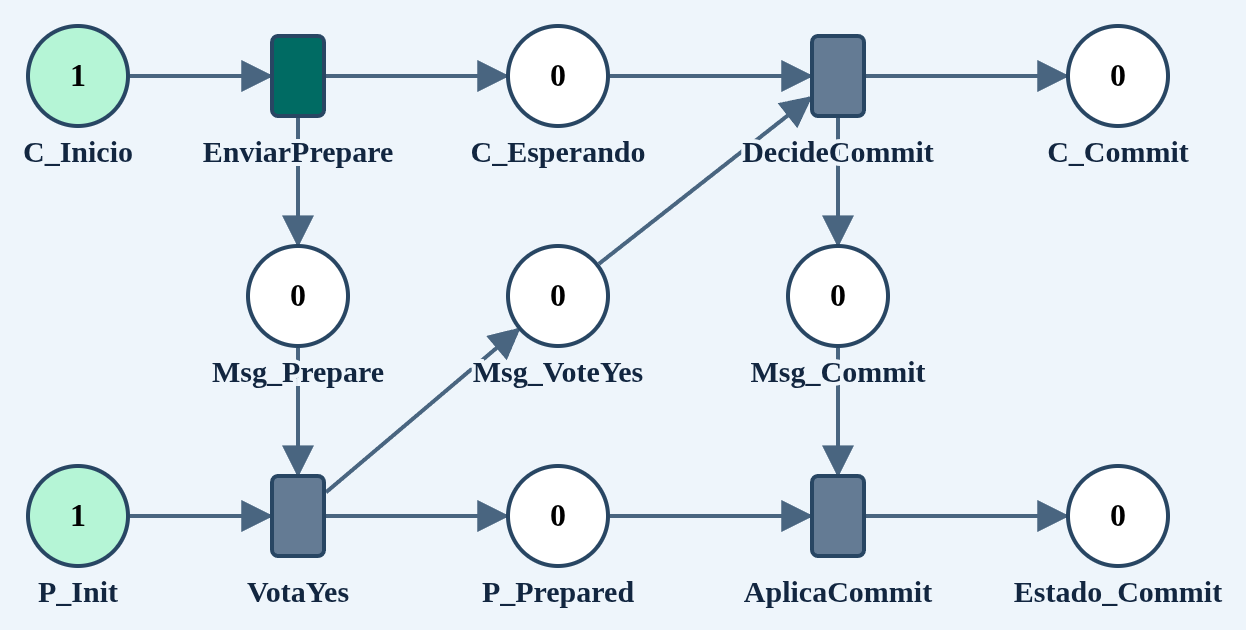
\includegraphics[width=\textwidth]{../diagrama_petri_2pc.png}
    \caption{Red de Petri del protocolo 2PC con un participante.}
    \label{fig:red-petri-2pc}
\end{figure}

\subsection{Lugares y transiciones}

Los lugares principales de la red son:

\begin{itemize}
    \item \texttt{Coordinador\_Inicio}, \texttt{Coordinador\_Esperando\_Votos},
    \texttt{Coordinador\_Commit}, \texttt{Coordinador\_Rollback} y
    \texttt{Coordinador\_Caido}, que representan el estado del coordinador.
    \item \texttt{Participante\_Init}, \texttt{Participante\_Prepared},
    \texttt{Estado\_Commit} y \texttt{Estado\_Rollback}, que representan el
    estado del participante.
    \item \texttt{Msg\_Prepare}, \texttt{Msg\_VoteYes},
    \texttt{Msg\_VoteNo}, \texttt{Msg\_Commit} y
    \texttt{Msg\_Rollback}, que representan mensajes enviados pero todavía no
    consumidos.
\end{itemize}

La marcación inicial tiene un token en
\texttt{Coordinador\_Inicio} y otro en \texttt{Participante\_Init}. La
ejecución exitosa queda descrita por la siguiente secuencia:

\begin{enumerate}
    \item \texttt{EnviarPrepare} mueve el token del coordinador a
    \texttt{Coordinador\_Esperando\_Votos} y genera un token en
    \texttt{Msg\_Prepare}.
    \item \texttt{VotaYes} consume \texttt{Msg\_Prepare} y el token de
    \texttt{Participante\_Init}; deja al participante en
    \texttt{Participante\_Prepared} y genera \texttt{Msg\_VoteYes}.
    \item \texttt{DecideCommit} consume el token de
    \texttt{Coordinador\_Esperando\_Votos} y \texttt{Msg\_VoteYes}; deja al
    coordinador en \texttt{Coordinador\_Commit} y genera
    \texttt{Msg\_Commit}.
    \item \texttt{AplicaCommit} consume \texttt{Participante\_Prepared} y
    \texttt{Msg\_Commit}; deposita el token final en
    \texttt{Estado\_Commit}.
\end{enumerate}

La rama alternativa usa \texttt{VotaNo} y
\texttt{DecideRollback}, y termina en \texttt{Estado\_Rollback}; no es
habilitable al mismo tiempo que la rama exitosa porque ambas requieren el
token único de \texttt{Msg\_Prepare} y del estado inicial del participante.

\subsection{Invariante de lugar}

Sea $M(p)$ la cantidad de tokens del lugar $p$. El siguiente invariante de
lugar expresa que el participante solo puede encontrarse en uno de sus
estados:

\[
 M(\texttt{Participante\_Init})+
 M(\texttt{Participante\_Prepared})+
 M(\texttt{Estado\_Commit})+
 M(\texttt{Estado\_Rollback})=1.
\]

El valor inicial es $1$. Cada transición que cambia el estado del
participante consume exactamente el token del estado actual y produce
exactamente un token en el estado siguiente. Por lo tanto, el valor se
conserva en toda marcación alcanzable. En particular, si
$M(\texttt{Estado\_Commit})=1$, entonces
$M(\texttt{Estado\_Rollback})=0$, y viceversa. Así se demuestra
matemáticamente que una transacción no puede quedar confirmada y revertida
simultáneamente.

\subsection{Acotamiento y seguridad}

Una red es \emph{1-acotada} (o \emph{safe}) si, desde la marcación inicial y
para toda ejecución posible, ningún lugar puede contener más de un token.
En este modelo, esto significa que:

\begin{itemize}
    \item hay como máximo una instancia de la transacción modelada en cada
    estado del coordinador y del participante;
    \item no se duplican los mensajes de una misma fase; y
    \item el participante no puede acumular dos decisiones finales ni
    mantener simultáneamente los estados \texttt{Commit} y
    \texttt{Rollback}.
\end{itemize}

La 1-acotación es una propiedad de seguridad del negocio: evita que una
misma reserva se confirme dos veces, que se revierta dos veces o que existan
dos decisiones incompatibles para la misma transacción. No implica que la
transacción siempre termine; por ejemplo, la red puede quedar esperando si
el coordinador cae antes de enviar una decisión.
